\chapter{Phénomène de localisation d'Anderson} 
\label{ch:Localisation}
%\begin{tikzpicture}[remember picture, overlay]
%\node[anchor=north east,inner sep=0pt] at (current page.north east) {
\includegraphics[scale=1]{Fig/Localisation/g825.png}};
%\end{tikzpicture}

Dans ce chapitre, nous commencerons par décrire comment, lors de la propagation cohérente d'une onde dans un milieu désordonné, les interférences peuvent altérer la diffusion classique et engendrer le phénomène spectaculaire de \emph{Localisation d'Anderson} dont nous donnerons les principales propriétés. Dans un second temps, nous présenterons succinctement les principaux systèmes utilisés pour l'investigation de la localisation d'Anderson, pour s'attarder plus particulièrement sur les expériences d'atomes froids. Enfin, nous terminerons ce chapitre par une discussion de nos enjeux actuels, l'étude du régime critique de la transition d'Anderson avec des atomes froids, dont nous présenterons l'état de l'art.

\section{Diffusion et interférences}
Cette première section a pour but de rappeler succinctement les mécanismes microscopiques à l'œuvre lors de l'étude de la propagation d'une onde dans un milieu désordonné, et comment le phénomène d'interférence peut modifier les grandeurs microscopiques associées. En particulier, nous nous focaliserons sur l'arrêt de la diffusion en conséquence de ces interférences, la localisation d'Anderson.

\subsection{Phénomène de diffusion}
\label{sc:diffusion_classique}
Le phénomène de diffusion macroscopique est un des phénomènes de transport les plus connus de la physique classique. Celui-ci permet par exemple de décrire de manière simple et unifiée la propagation de la chaleur dans un matériau homogène, l'homogénéisation de la concentration de particules dans un liquide ou encore le phénomène de résistance électrique. 

Le phénomène macroscopique de diffusion provient, de manière générale, de la marche aléatoire de particules au sein de leur environnement. Avec cette approche, Drude a par exemple été le premier à calculer la résistivité électrique des matériaux en introduisant un temps de relaxation microscopique basé sur des collisions élastiques entre les électrons, vecteurs du courant électrique, et les impuretés du matériau dans lequel ceux-ci se déplacent \citep{ashcroft2010solid}. 

Cet exemple historique illustre le fait que certaines propriétés macroscopiques des matériaux sont reliées aux grandeurs microscopiques de la marche aléatoire associée. Ces dernières grandeurs sont des briques élémentaires de la propagation en milieu désordonné, dont nous restreindrons l'étude au cas des collisions élastiques entre les particules et le désordre. Parmi ces briques élémentaires, que nous présenterons dans la suite, nous retrouvons le coefficient de diffusion, le temps de transport, ou encore le temps de diffusion élastique, auquel nous porterons une attention particulière.

\paragraph*{Temps de diffusion élastique}
La quantité la plus naturelle permettant de caractériser de manière microscopique le phénomène de diffusion est le \emph{temps de diffusion élastique} $\taus$, qui correspond à la durée typique entre deux évènements successifs de \emph{collision élastique} avec les impuretés du milieu. Ce temps est l'équivalent temporel du \emph{libre parcours moyen}  $\ls$ correspondant à la distance moyenne entre deux évènements de diffusion microscopiques successifs, illustrée figure \ref{fig:diffusion_classique}.a. Dans le cas d'une particule de masse $m$ se déplaçant à une vitesse $v_{\mathrm{i}}$, ces deux grandeurs sont reliées par
\begin{equation}
\taus=\frac{\ls}{v_{\mathrm{i}}}=\frac{m}{\hb} \frac{\ls}{k_{\mathrm{i}}} \text{ ,}
\label{eq:definition_taus}
\end{equation}
où $k_{\mathrm{i}}$ est le nombre d'onde de l'onde quantique associée à la particule (celui-ci est inchangé après chaque évènement de collision en raison de leur caractère élastique). 

Comme nous le verrons plus en détails dans les chapitres \ref{ch:TauS_PRL} et \ref{ch:TauS_NJP}, le temps de diffusion élastique est une quantité qui dépend des détails microscopiques du système et peut être interprété comme le temps de vie d'une onde plane dans le désordre.

\paragraph*{Temps de transport}
Si la norme du vecteur vitesse (ou de manière équivalente du vecteur d'onde) reste inchangée au cours de la propagation, sa direction est modifiée à chaque évènement de collision élastique. Comme nous le verrons plus en détails dans le chapitre \ref{ch:TauS_PRL}, lors de la collision avec un diffuseur de taille caractéristique $\sigma$, l'onde peut être diffusée selon un angle typique $\theta_{\mathrm{typ}}\sim 1/k_{\mathrm{i}} \sigma$. La diffusion peut donc être \emph{anisotrope}, en analogie avec la diffusion de Mie ou la diffraction en optique.

En considérant que la trajectoire d'une particule est composée de multiples collisions successives, il apparaît alors une seconde échelle de temps caractéristique, le \emph{temps de transport} ou temps de Boltzmann $\taub$, décrivant la durée nécessaire pour que la particule perde l'information de la direction initiale de sa vitesse. 


On peut ainsi montrer que le temps de transport (et son analogue spatial, la \emph{longueur de transport}) s'expriment en fonction du temps de diffusion élastique de la manière suivante \citep{akkermans2007mesoscopic}:
\begin{equation}
\taub=\frac{\taus}{1-\left\langle\cos{\theta}\right\rangle} \quad \text{et} \quad \lb=\frac{\ls}{1-\left\langle\cos{\theta}\right\rangle} \text{ ,}
\label{eq:definition_taub}
\end{equation}
où $\langle\:\cdots\:\rangle$ représente la valeur moyenne sur les différents évènements de diffusion, et $\theta$ l'angle de diffusion comme indiqué sur la figure \ref{fig:diffusion_classique}.a.

On voit donc que dans le cas de collisions élastiques isotropes, $\taub=\taus$, montrant qu'une seule collision suffit à perdre l'information sur la direction initiale de la vitesse de la particule. En revanche, un grand nombre de collisions sont nécessaires pour obtenir une isotropisation de la direction des vitesses dans le cas d'évènements de diffusion anisotrope.


\begin{figure}
\centering
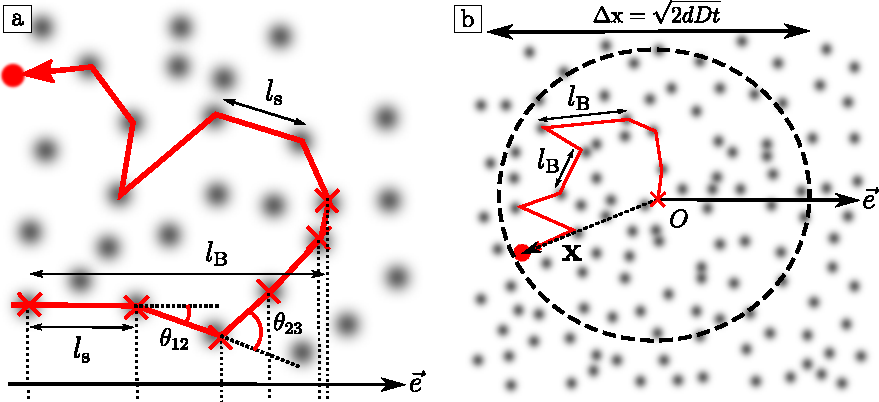
\includegraphics[width=\textwidth]{Fig/Localisation/diffusion_classique.pdf}
\caption{\textbf{a: Longueur de transport pour des collisions anisotropes.} Dans le cas de diffusion fortement anisotrope vers l'avant, une unique collision élastique ne modifie que peu la direction de la vitesse d'une particule. Il faut donc un grand nombre de collisions successives pour que la direction de la vitesse d'une particule soit décorrélée de la direction initiale. En conséquence, le temps de transport est beaucoup plus grand que le temps de diffusion élastique. \textbf{b: Mécanisme microscopique de la diffusion.} Le mouvement d'une particule peut être considérée comme une marche aléatoire composée d'évènements de diffusion isotropes tous les $\taub$ entre lesquels la particule se déplace d'une distance $\lb=v \taub$ dans une direction aléatoire. L'étalement typique obtenu croit avec le temps selon $\Delta \mathrm{x} =\sqrt{2dDt}$, avec $D$ le coefficient de diffusion.}
\label{fig:diffusion_classique}
\end{figure}





\paragraph*{Coefficient de diffusion}
Une fois que la particule a parcouru une distance $\lb$, on peut considérer qu'elle subit une diffusion isotrope. On assimile alors le mouvement des particules à une marche aléatoire pour laquelle les particules de vitesse $v$ subissent des évènements de collision isotrope à chaque intervalle de temps $\taub$ pendant lesquels la particule parcourt une distance $\lb=v \taub$, comme illustré figure \ref{fig:diffusion_classique}.b.

Ainsi, on peut déterminer l'étalement typique de la région explorée par la particule après $N$ collisions\footnote{On peut montrer que la probabilité qu'une particule ne subisse pas de collision isotrope sur une distance $x$ est donnée par $\mathcal{P}_x(x)=\frac{1}{\lb} e^{-x/\lb}$. La variance est alors obtenue par $\langle\Delta x^2 \rangle = \int_0^\infty{\diff x \: x^2 \:  \mathcal{P}_x(x)}=2\lb^2 $. Les $N$ collisions successives étant décorrélées, l'étalement typique de la région explorée est alors de $N \langle\Delta x^2 \rangle$.},
\begin{equation}
\left\langle \Delta \mathbf{x}^2 \right\rangle=2 N \lb^2 \text{ .}
\end{equation}
En définissant le coefficient de diffusion par $ \left\langle \Delta \mathbf{x}^2 \right\rangle = 2 d D t$ et en faisant apparaître le temps $t=N \taub$, on montre ainsi que \citep{akkermans2007mesoscopic}:
\begin{equation}
D=\frac{v \lb}{d}=\frac{\hb}{m d} k \lb \text{ ,}
\label{eq:definition_coefficient_diffusion}
\end{equation}
en faisant apparaître la quantité $k \lb$, qui sera essentielle dans la suite. Cette quantité peut être interprétée comme une mesure de la force du désordre comme nous aurons l'occasion de le voir dans la section \ref{sc:localisation_anderson} et dans le chapitre \ref{ch:TauS_PRL}. Notamment, le régime de désordre faible est défini par la condition $k\lb\gg 1$, signifiant que la distance entre deux collisions isotropes successives est très grande devant la longueur d'onde.

Une conséquence de l'équation \ref{eq:definition_coefficient_diffusion} est qu'une diminution de la longueur de transport entraîne une diminution du coefficient de diffusion. Ainsi, plus un système sera désordonné, plus le coefficient de diffusion sera petit.














\subsection{Localisation faible}
\label{sc:weak_localisation}
Si le mécanisme de marche aléatoire présenté permet de décrire un grand nombre de situations de diffusion classique, nous avons omis un ingrédient essentiel à la propagation d'ondes en milieu désordonné: la \emph{cohérence}, ou encore la capacité qu'une onde a à interférer. En particulier, nous verrons que celle-ci peut avoir des conséquences dramatiques sur les propriétés de transport d'une onde en présence de désordre.

\paragraph*{Mécanisme de localisation faible}
Pour cela, intéressons-nous à la probabilité $P(\mathbf{x},\mathbf{x}')$ qu'une onde initialement à la position $\mathbf{x}$ se retrouve à la position $\mathbf{x}'$ après propagation dans le milieu désordonné. Dans la limite $k\lb\gg 1$, la trajectoire de l'onde peut être vue comme une marche aléatoire, où chaque trajectoire de diffusion est associée à une amplitude complexe de probabilité $\left| A_j \right| e^{i \phi_j}$, avec $\phi_j$ la phase de la trajectoire. Ainsi, la probabilité $P(\mathbf{x},\mathbf{x}')$ est donnée par la somme de l'amplitude sur toutes les trajectoires possibles:
\begin{align}
P(\mathbf{x},\mathbf{x}') \nonumber&= \overline{{\left| \sum_j{ \left|A_j\right| e^{i \phi_j} }\right| }^2} = \overline{\sum_{j,l} {\left| A_j \right| \left| A_l \right| e^{i (\phi_j - \phi_l)}}} \\
&= \overline{\sum_j{{\left| A_j \right|}^2}} + \overline{\sum_{j\neq l}{\left| A_j \right| \left|A_l \right| e^{i(\phi_j - \phi_l)}}} \text{ ,}
\label{eq:amplitude_localisation_faible}
\end{align}
où $\overline{\:\cdots\:}$ désigne la moyenne sur les différentes réalisations du désordre.

Le premier terme décrit le phénomène de diffusion classique, pour lequel la probabilité $P(\mathbf{x},\mathbf{x}')$ est la somme des probabilités de chaque trajectoire. 

Le second terme de l'équation \ref{eq:amplitude_localisation_faible} représente quant à lui les interférences dues aux différentes phases accumulées par les différents chemins de diffusion. Intuitivement, on peut considérer que la contribution de ce terme s'annule en moyennant sur les différentes réalisations du désordre, $\overline{e^{i(\phi_j - \phi_l)}}=0$\footnote{L'annulation de ce second terme est à l'origine du traitement classique de la propagation d'ondes dans le désordre tels que dans la théorie de Drude ou du transfert radiatif.}. Cependant, une étude attentive montre que certaines trajectoires résistent au moyennage sur les réalisations du désordre.

En particulier, les trajectoires pour lesquelles l'onde se retrouve à son point de départ forment des boucles qu'il est possible de parcourir dans les deux sens, comme illustré figure \ref{fig:localisation_faible}. Par \emph{symétrie par renversement du temps}, la phase accumulée le long de ces trajectoires est identique pour les deux sens de propagation. De plus, ces paires de trajectoires existent quelque soit la réalisation du désordre, rendant ce processus d'interférences constructives robuste vis-à-vis du moyennage d'ensemble et $\overline{e^{i(\phi_j - \phi_l)}}=1$. Ainsi, la probabilité qu'une onde retourne à son point de départ est le double de la prédiction classique:
\begin{equation}
P(\mathbf{x},\mathbf{x})=2 \overline{\sum_j{{\left| A_j \right|}^2}} \text{ .}
\label{eq:proba_retour_origine}
\end{equation}

Les interférences entre chemins de diffusion tendent alors à favoriser le retour de l'onde à son point d'origine, ralentissant ainsi la diffusion. Cet effet de \emph{localisation faible}, commun à tout type d'onde, a été intensivement étudié aussi théoriquement que expérimentalement dans de nombreux domaines, tels qu'en physique des solides \citep{kramer1993localization}\citep{akkermans2007mesoscopic}, en optique \citep{wolf1985weak}\citep{mishchenko1993nature}, avec des ondes sismiques \citep{larose2004weak} ou encore avec des atomes froids \citep{jendrzejewski2012coherent}\citep{muller2015suppression}.


\begin{figure}
\centering
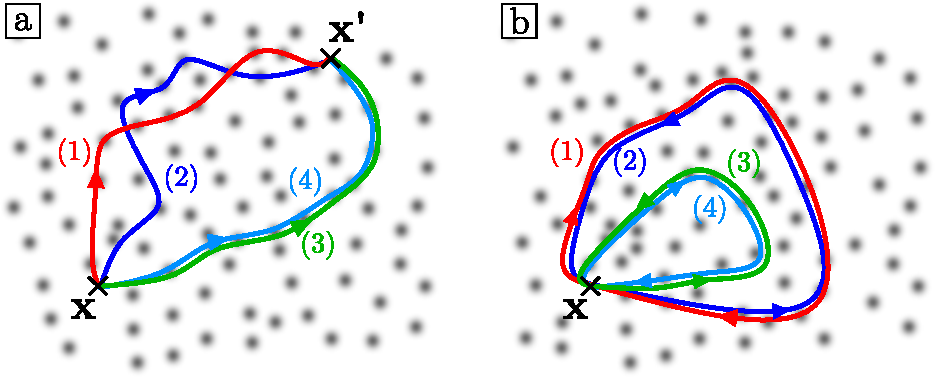
\includegraphics[width=0.9\textwidth]{Fig/Localisation/localisation_faible.pdf}
\caption{\textbf{a: Participation des différents chemins de diffusion à la propagation de l'onde.} La probabilité d'arriver au point $\mathrm{x'}$ en partant du point $\mathrm{x}$ est donnée par l'ensemble des trajectoires les reliant. Dans le cas des chemins 1 et 2, la phase accumulée le long de ces trajectoires diffère, détruisant en moyenne le phénomène d'interférence entre ces chemins. \textbf{b: Mécanisme de localisation faible.} Les chemins de diffusion pour lesquels l'onde retourne à son point de départ se présentent sous forme de boucles qu'il est possible de parcourir dans les deux sens, comme illustré par les trajectoires 1 et 2, ou encore les trajectoires 3 et 4. Ces paires de trajectoires existent quelle que soit la réalisation du désordre.}
\label{fig:localisation_faible}
\end{figure}



\paragraph*{Corrections de localisation faible}
Comme le montre l'équation \ref{eq:proba_retour_origine}, le retour de l'onde à son point d'origine est favorisé à l'aide des interférences constructives qu'il existe entre des trajectoires symétriques par renversement du temps. Notamment, cet effet de localisation faible se traduit par la diminution du coefficient de diffusion par rapport à la prédiction classique \ref{eq:definition_coefficient_diffusion}, que l'on peut alors écrire sous la forme
\begin{equation}
D= D_{\mathrm{0}}-\delta D \text{ ,}
\end{equation}
où $D_{\mathrm{0}}$ est le coefficient de diffusion classique \ref{eq:definition_coefficient_diffusion}, et $\delta D$ est la correction de localisation faible. Ces corrections de localisation faible dépendent des détails microscopiques du système, mais aussi de sa dimension $d$ et de sa taille $L$. En estimant le poids des boucles de localisation faible, on peut montrer que \citep{akkermans2007mesoscopic}:
\begin{equation}
\delta D/ D_{\mathrm{0}} = \left\lbrace \begin{aligned}
& \mathcal{O}\left(L/l_{\mathrm{B}}\right)  \quad &&\text{en 1D ,}\\
& \mathcal{O}\left(\frac{1}{k l_{\mathrm{B}}} \ln{\frac{L}{l_{\mathrm{B}}}} \right) \quad &&\text{en 2D ,}\\
& \mathcal{O}\left(\frac{1}{(k l_{\mathrm{B}})^2}\right) \quad &&\text{en 3D .}
\end{aligned}\right.
\label{eq:correction_localisation_faible}
\end{equation}
Ces relations témoignent ainsi de la forte influence de la dimension du système comme nous le verrons plus en détails dans la section suivante.






\subsection{Suppression du transport: Localisation d'Anderson}
\label{sc:localisation_anderson}

Les corrections de localisation faible données par l'équation \ref{eq:correction_localisation_faible} font apparaître un comportement remarquable: sous certaines conditions, il est possible que la correction $\delta D$ soit égale au coefficient de diffusion classique $D_{\mathrm{0}}$, entraînant ainsi la suppression du transport avec $D=0$. Cet effet dit de \emph{Localisation forte}, ou encore de \emph{Localisation d'Anderson}, a été découvert en 1958\footnote{Le phénomène de localisation d'Anderson a été découvert avant les processus de localisation faible.} par \emph{Philip W. Anderson} s'intéressant alors à la diffusion d'une particule quantique dans un réseau désordonné dans le cadre de la physique de la matière condensée \citep{anderson1958absence}. Cette inhibition du transport constitue la signature la plus spectaculaire de l'influence de la cohérence de l'onde lors de sa propagation dans un milieu désordonné. Ces travaux furent récompensés par le prix Nobel de physique en 1977, conjointement avec \emph{Sir Nevill Francis Mott} et \emph{John Hasbrouck van Vleck}. 



\paragraph*{Localisation d'Anderson et rôle de la dimension}
Dans le régime \emph{isolant}\footnote{Par opposition au régime \emph{métallique} où le transport existe.} de localisation d'Anderson, la fonction d'onde reste localisée aux alentours du point d'origine et présente un profil exponentiel
\begin{equation}
\left| \psi (\mathbf{x}) \right|^2 \propto e^{-\mathrm{x}/\xiloc} \text{ ,}
\label{eq:exponentielle_anderson}
\end{equation}
où $\xiloc$ correspond à la longueur typique sur laquelle l'onde s'étend, et est appelée \emph{longueur de localisation}\footnote{La longueur de localisation est définie comme la longueur caractéristique de décroissance des ailes de la fonction d'onde moyenne $\xiloc=\lim\limits_{x\rightarrow\infty} -\frac{x}{\;\overline{\ln|\psi(x)|^2}\;}$.}.

Pour un système de taille suffisamment grande, les corrections de localisation faible $\delta D$ de l'équation \ref{eq:correction_localisation_faible} en dimension 1 sont du même ordre que le coefficient de diffusion classique $D_{\mathrm{0}}$. On constate ainsi qu'en dimension 1, les processus de localisation faible sont très efficaces, rendant tous les états localisés. Il est possible d'estimer la longueur de localisation à l'aide des corrections de localisation faible en écrivant $\delta D(\xiloc)\sim D_{\mathrm{0}}$, d'où on déduit que $\xiloc=2 \lb$ pour un système unidimensionnel. De fait, la localisation d'Anderson se manifeste même pour des désordres faibles, témoignant de son caractère spectaculaire. 


De même, à deux dimensions, il apparaît des corrections de localisation faible \ref{eq:correction_localisation_faible} que tous les états sont localisés pour un système de taille suffisamment grande. En écrivant $\delta D(\xiloc)\sim D_{\mathrm{0}}$, on trouve ainsi que les états restent localisés mais sur des échelles de longueurs bien plus grandes que dans le cas unidimensionnel, de l'ordre de $\xiloc \sim \lb \exp{(k \lb)}$. Pour des désordres faibles ($k \lb \gg 1$), la longueur de localisation excède généralement la taille du système. On parle ainsi de dimension \emph{marginale} de la localisation d'Anderson.

Remarquablement, les corrections de localisation faible à trois dimensions ne dépendent pas de la taille du système, mais seulement de la force du désordre $k \lb$. Dans le cas d'un désordre faible ($k\lb\gg 1$), les boucles de localisation faible ne sont pas assez nombreuses pour changer de manière significative la dynamique diffusive de l'onde ($\delta D \ll D_{\mathrm{0}}$). En revanche, la localisation d'Anderson persiste dans le cas d'un désordre fort où $k \lb \leq 1$, pour lequel la phase de l'onde varie peu entre deux évènements successifs de diffusion. 

Notons que l'analyse intuitive des propriétés de localisation en fonction de la dimension à l'aide des corrections de localisation faible présentée ici a été rigoureusement étudiée et validée dans le cadre de la \emph{théorie d'échelle de la localisation d'Anderson}, développée à la fin des années 1970 \citep{abrahams1979scaling}.

\paragraph*{Transition d'Anderson à trois dimensions}
Il apparaît donc que le cas à trois dimensions présente un intérêt particulier. En effet, un même système peut, selon la force du désordre, présenter un comportement qui soit métallique ou isolant. Selon l'équation \ref{eq:correction_localisation_faible}, on peut estimer que ce changement de comportement se manifeste lorsque
\begin{equation}
k \lb \sim 1 \text{ ,}
\label{eq:ioffe_regel}
\end{equation}
condition connue sous le nom de \emph{critère de Ioffe-Regel}. 

Il est possible de donner une interprétation intuitive au critère de Ioffe-Regel en se focalisant sur la phase accumulée par l'onde entre deux évènements successifs de diffusion. En effet, cette phase est de l'ordre de $\phi\sim k\lb$. Dans le régime de désordre fort, la phase de l'onde est donc similaire pour plusieurs évènements de diffusion successifs, générant ainsi des interférences constructives entre les différentes ondes diffusées. 

Plus particulièrement, il a été montré à l'aide la théorie d'échelle de la localisation d'Anderson qu'il existe une transition de phase du deuxième ordre entre états localisés et états diffusifs pour des systèmes à trois dimensions \citep{abrahams1979scaling}. Le paramètre de contrôle de la transition étant l'énergie $E$ de l'onde, la transition d'Anderson possède donc une énergie critique $\Ec$ appelée \emph{seuil de mobilité}, comme illustré figure \ref{fig:transition_anderson}.a. 

La transition d'Anderson est de plus caractérisée par deux exposants critiques $\nu$ et $s$, décrivant respectivement comment la longueur de localisation $\xiloc$ diverge pour des états localisés proches du seuil de mobilité et comment le coefficient de diffusion $D$ s'approche de $0$ pour des états diffusifs (voir figure \ref{fig:transition_anderson}.b):
\begin{equation}
D \sim \left| E-\Ec \right|^s \quad \text{et} \quad \xi_{\mathrm{loc}} \sim \left| E-\Ec \right|^{-\nu} \text{ .}
\end{equation}
Bien qu'aucune théorie ne puisse décrire exactement le régime critique de la transition d'Anderson à l'heure actuelle, plusieurs études numériques s'accordent sur les valeurs $s=\nu=1.58$ des exposants critiques \citep{slevin1999corrections} \citep{evers2008anderson} \citep{slevin2014critical}. À ce jour, seule une expérience \textit{indirecte} a été capable de mesurer ces exposants critiques (voir section \ref{sc:localisation_atomes_froids}) \citep{lopez2012experimental}


\begin{figure}
\centering
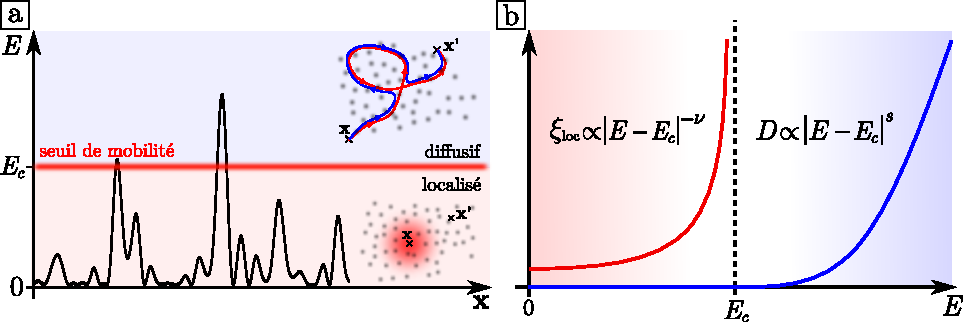
\includegraphics[width=\textwidth]{Fig/Localisation/transition_anderson.pdf}
\caption{\textbf{a: Transition d'Anderson.} À trois dimensions, il existe une transition de phase entre états diffusifs et états localisés. Pour une énergie supérieure à l'énergie critique de la transition, appelée seuil de mobilité, l'onde peut diffuser, tandis que pour une énergie inférieure au seuil de mobilité, l'onde est localisée. \textbf{b: Régime critique.} La transition d'Anderson est caractérisée par les exposants critiques $s$ et $\nu$, qui décrivent comment évoluent la longueur de localisation et la coefficient de diffusion aux alentours du seuil de mobilité. Dans le régime critique localisé, la longueur de localisation diverge en s'approchant du seuil de mobilité avec un exposant $\nu$. Dans le régime critique diffusif, le coefficient de diffusion s'annule selon une loi de puissance d'exposant $s$. }
\label{fig:transition_anderson}
\end{figure}
%\subsection{Théorie d'échelle}















\section{Localisation des atomes froids}
La localisation d'Anderson étant due au caractère ondulatoire du système étudié, celle-ci est donc commune à tout type d'onde, qu'elle soit classique (ondes lumineuses ou acoustiques) ou quantique (ondes électroniques, ondes de matière). Ce phénomène a donc été étudié expérimentalement à l'aide d'un grand nombre de systèmes dont nous allons brièvement présenter les principaux résultats ici, en mettant l'accent sur la transition métal-isolant.

\subsection{Etudes expérimentales de la localisation d'Anderson}
L'étude expérimentale de la localisation d'Anderson constitue un domaine de recherche qui s'est énormément développé, débutant dans les années 70-80 avec des systèmes électroniques et faisant aujourd'hui encore l'objet de recherches intenses.

\paragraph*{Localisation dans les systèmes électroniques}
Les premières expériences furent menées à l'aide de systèmes électroniques, et purent démontrer des effets de localisation faible ainsi que des effets de localisation forte \citep{mott1979electronic}\citep{paalanen1983critical}. Rapidement, les efforts se sont concentrés sur l'observation de la transition métal-isolant\footnote{Cette dénomination prend tout son sens dans les systèmes électroniques: les expériences menées correspondent à des mesures de conductivité.} prédite par la théorie d'échelle de la localisation. 

Cependant, une étude quantitative de la transition s'est révélée ardue en raison de la complexité de ces systèmes. En particulier, la présence d'interactions coulombiennes entre les électrons modifie profondément les propriétés de localisation, et rend délicate la distinction expérimentale entre la transition métal-isolant liée au désordre (transition d'Anderson) et la transition métal-isolant liée aux interactions (transition de Mott). Ces effets sont particulièrement marqués par la comparaison entre les exposants critiques mesurés ($\nu\sim 1$ pour \citep{shlimak1996determination}) et ceux estimés à l'aide de simulations numériques ($\nu\sim1.58$). Notons tout de même que de nouvelles expériences rapportent l'observation de la localisation d'Anderson à l'aide systèmes électroniques \citep{siegrist2011disorder}\citep{ying2016anderson}.


\paragraph*{Localisation dans les systèmes classiques} 
L'utilisation des ondes classiques s'est alors imposée comme étant un moyen de réaliser des systèmes mieux contrôlés que dans le cadre de la matière condensée. Les premières signatures de la localisation d'Anderson ont été obtenues dans les années 90 avec des ondes ultrasonores \citep{weaver1990anderson}, des ondes mécaniques de flexion \citep{ye1992observation}, des micro-ondes \citep{genack1991observation} ainsi que des ondes lumineuses \citep{wiersma1997localization}. 

Cependant, ces premières expériences s'appuyaient sur la décroissance exponentielle de l'intensité de l'onde pour analyser leurs résultats. Leur interprétation fut controversée en raison de l'existence d'autres phénomènes présentant la même signature, en particulier l'absorption qui présente aussi une décroissance exponentielle de l'intensité de l'onde comme décrit par la loi de Beer-Lambert \citep{scheffold1999localization}. Depuis, d'autres signatures ont été exploitées telle que la dynamique de l'onde en régime pulsé \citep{weaver1993anomalous} ou encore les fluctuations géantes de transmission \citep{nieuwenhuizen1995intensity} afin d'observer sans ambiguïté la localisation d'Anderson.

Aujourd'hui encore, la difficulté expérimentale s'accroît fortement en augmentant la dimension du système. En particulier, augmenter le pouvoir diffusant du milieu à trois dimensions afin d'atteindre le critère de Ioffe-Regel $k \lb \sim 1$ tout en s'affranchissant de l'absorption reste un tour de force expérimental. Ainsi, la seule observation de la localisation d'Anderson à trois dimensions faisant consensus à été réalisée au Canada dans le groupe de J. Page à l'aide d'ondes acoustiques se propageant dans des billes d'aluminium \citep{hu2008localization}.

Notons finalement que la localisation à trois dimensions d'ondes lumineuses fait l'objet de recherches intenses très débattues. Enfin, une récente étude numérique prédit l'absence de la localisation d'Anderson à trois dimensions dans le cas d'ondes lumineuses en raison de leur caractère vectoriel \citep{skipetrov2014absence}.





\begin{figure}
\centering
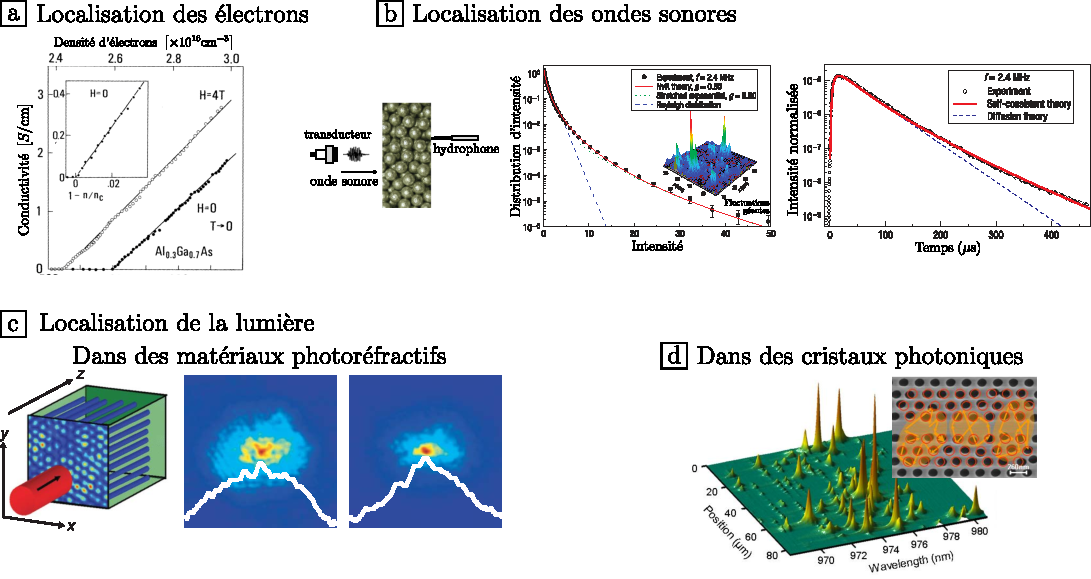
\includegraphics[width=\textwidth]{Fig/Localisation/experiences_localisation_anderson.pdf}
\caption{\textbf{Etudes expérimentales de la localisation d'Anderson.} \textbf{a:} A basse température, un métal peut devenir isolant à cause du désordre, sa conductivité s'annulant alors. Cette transition peut être atteinte en diminuant la densité d'électrons. Figure tirée de \citep{katsumoto1987fine}. \textbf{b:} La localisation d'Anderson d'ondes élastiques dans un réseau désordonné de billes d'aluminium peut être étudiée à l'aide d'un hydrophone après sa propagation. Il est possible de relever la distribution d'intensité de l'onde ainsi que son profil temporel qui présentent des signatures de la localisation d'Anderson. Figures tirées de \citep{hu2008localization}. \textbf{c} et \textbf{d:} La localisation de la lumière peut être étudiée à l'aide de plusieurs systèmes, tels que des matériaux photoréfractifs composés d'un réseau désordonné de guides d'ondes (\textbf{c}, figure tirée de \citep{schwartz2007transport}) ou encore dans des cristaux photoniques (\textbf{d}, figure tirée de \citep{sapienza2010cavity}).}
\label{fig:experiences_localisation_anderson}
\end{figure}






\subsection{L'approche des atomes froids}
\label{sc:localisation_atomes_froids}
Depuis le milieu des années 2000, une nouvelle plateforme participe à l'étude de la physique du désordre: les atomes ultra-froids. Ces systèmes, utilisés en interférométrie atomique et pour de la simulation quantique, sont bien connus pour leurs propriétés de cohérence sous forme de \emph{condensats de Bose-Einstein}. Ceux-ci présentent un degré de contrôle inédit et offrent des possibilités expérimentales complexes qu'il est impossible d'obtenir à l'aide d'autres systèmes.

En effet, les expériences d'atomes ultra-froids présentent un grand nombre d'avantages: il est possible d'imager la fonction d'onde des atomes aussi bien dans l'espace réel grâce à une imagerie \emph{in-situ} que dans l'espace des vitesses à l'aide d'une imagerie par \emph{temps de vol}. De plus, les atomes ultra-froids ne présentent pas d'absorption, et dépassent ainsi les difficultés des expériences pionnières d'observation de la localisation d'Anderson. Enfin, de tels systèmes offrent un vaste contrôle des paramètres microscopiques, de l'onde comme du désordre en passant par la dimension. Les atomes ultra-froids apparaissent alors comme une plateforme idéale pour étudier la physique du désordre.


\paragraph*{Atomes ultra-froids et désordre}
Il existe différentes méthodes pour générer un désordre sur les atomes. Parmi les plus utilisées on retrouve les champs de tavelures optiques, ou \emph{speckle}, et les réseaux bichromatiques pour lesquels un réseau de faible amplitude vient moduler de manière quasi-aléatoire le réseau principal (voir figure \ref{fig:localisation_1D_atomes_froids}). Notons aussi le développement récent de désordres générés à l'aide de modulateurs spatiaux de lumière ou de matrices de micro-miroirs, permettant de réaliser des profils d'illumination arbitraires.

Toutes ces façons de réaliser un désordre pour les atomes possèdent un point commun: ils sont générés à l'aide de champs lumineux et possèdent donc une longueur typique de variation, ou \emph{longueur de corrélation} $\sigma$, généralement de l'ordre du micromètre. L'existence de cette longueur typique impose une température critique pour le système présente un comportement quantique. En particulier, les effets quantiques associés au comportement ondulatoire de la matière sont attendus lorsque la longueur de \emph{de Broglie} est plus grande que la longueur de corrélation:
\begin{equation}
\ldb\geq\sigma \quad \text{soit} \quad T_{\mathrm{typ}} \leq \frac{\hb^2}{ \kB m \sigma^2}\sim \text{ quelques nanokelvins.}
\end{equation}
L'observation d'effets quantiques en présence de désordre nécessite donc des températures extraordinairement basses qui sont typiquement obtenues avec des \emph{condensats de Bose-Einstein}. 

Cependant, l'obtention de telles températures n'est pas nécessaire pour observer la dynamique diffusive d'atomes dans un désordre optique. Notamment, celle-ci a été étudiée en deux dimensions en se concentrant sur la décroissance temporelle de la densité atomique \citep{robert2010anisotropic}. Plus particulièrement, une décroissance de la densité atomique en $1/t$ au centre du nuage servant de point source, signature de la dynamique diffusive, a été observée en présence de désordre, tandis que celle-ci est caractérisée par une décroissance en $1/t^2$ pour une expansion balistique en absence de désordre.



\begin{figure}
\centering
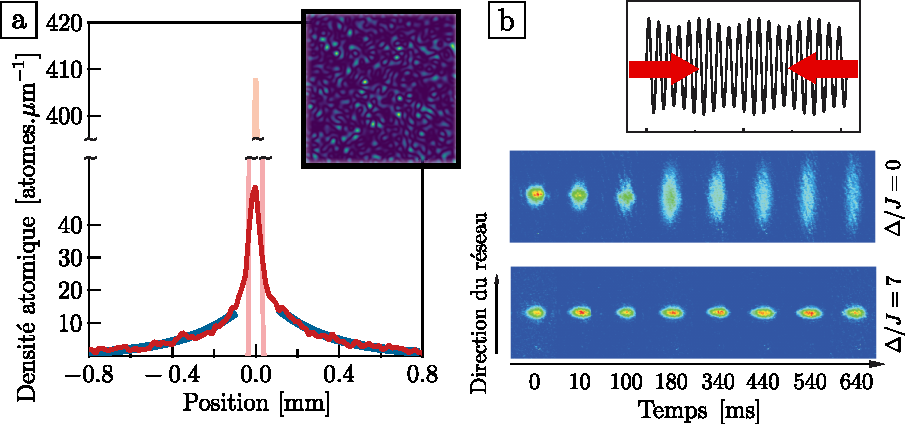
\includegraphics[width=\textwidth]{Fig/Localisation/localisation_1D_atomes.pdf}
\caption{\textbf{Premières expériences de localisation unidimensionnelle.} \textbf{a:} Localisation d'ondes atomiques dans un réseau bichromatique unidimensionnel. Un condensat de Bose-Einstein s'étend dans l'espace libre (image du haut), tandis que son expansion est arrêtée lorsque celui-ci est placé dans un potentiel quasi-périodique (image du bas). Figure tirée de \citep{roati2008anderson}. \textbf{b:} Localisation d'Anderson unidimensionelle d'ondes de matière dans un speckle. La densité atomique est mesurée après une seconde d'expansion dans un guide d'onde unidimensionnel et dans un potentiel de type speckle. Les ailes du profil sont caractérisées par un décroissance exponentielle (traits bleus). Le profil rose correspond à la densité atomique initiale. Figure tirée de \citep{billy2008direct}.}
\label{fig:localisation_1D_atomes_froids}
\end{figure}




\paragraph*{Localisation d'Anderson d'ondes atomiques}
C'est en 2008 qu'a été observée la localisation d'Anderson d'ondes de matière simultanément dans deux expériences illustrées sur la figure \ref{fig:localisation_1D_atomes_froids}. L'expérience de Roati et al. \citep{roati2008anderson} réalisée au LENS à Florence, rapporte l'arrêt de l'expansion d'un condensat de Bose-Einstein de \isotope[39]{K} placé dans un potentiel unidimensionnel composé d'un réseau bichromatique. La seconde expérience, menée au Laboratoire Charles Fabry à Palaiseau, rapporte aussi l'arrêt de l'expansion d'un condensat de Bose-Einstein de \isotope[87]{Rb} plongé dans un guide d'onde optique unidimensionnel et dans un désordre de type speckle \citep{billy2008direct}. De plus, la mesure du profil de densité atomique montre la décroissance exponentielle \ref{eq:exponentielle_anderson} de la fonction d'onde localisée, comme représenté figure \ref{fig:localisation_1D_atomes_froids}.b. 

Ces expériences ont ainsi démontré la pertinence des atomes ultra-froids pour l'étude des systèmes désordonnés, et ont déclenché ainsi de nombreux efforts expérimentaux pour l'étude de la localisation d'Anderson dans des systèmes de dimensions 2 et 3. 

Ce n'est que récemment (2019) que la localisation d'Anderson a pu être observée à l'aide d'atomes froids en raison de l'augmentation exponentielle de la longueur de localisation avec la faiblesse du désordre. White et al. rapportent ainsi l'observation de la localisation d'Anderson en deux dimensions à l'aide d'une expérience de transmission entre deux réservoirs, et témoignent du profil exponentiel de la fonction d'onde dans le canal désordonné \citep{white2019observation}. 



\paragraph*{Localisation d'Anderson en trois dimensions}

C'est principalement vers l'étude de la localisation d'Anderson à trois dimensions et plus particulièrement vers l'étude du régime critique que ce se sont concentrés les efforts expérimentaux après l'observation de la localisation unidimensionnelle. Un des facteurs expliquant ce développement en faveur du cas tridimensionnel par rapport au cas bidimensionnel provient de la distinction entre la localisation d'Anderson, d'origine quantique, et le piégeage classique. Notamment, il a été montré que pour un potentiel de type speckle à trois dimensions, la percolation classique est négligeable \citep{pilati2010dilute}, contrairement au cas bidimensionnel où cette question est critique.

Trois expériences rapportent ainsi l'observation de la localisation d'Anderson à trois dimensions. Le groupe de B. de Marco à Urbana Champaign a ainsi utilisé un gaz fermionique de \isotope[40]{K} dans un potentiel speckle anisotrope \citep{kondov2011three}. Simultanément, l'équipe de Palaiseau a observé un arrêt de l'expansion d'une partie du nuage d'atomes de \isotope[87]{Rb} plongé dans un désordre isotrope généré par la superposition cohérente de deux speckles, pour des durées d'observation allant jusqu'à \SI{6}{\second} \citep{jendrzejewski2012three}. Enfin, une expérience récente menée au LENS dans l'équipe de G. Modugno rapporte l'observation de la localisation complète du nuage atomique de \isotope[39]{K}, dont les interactions ont été annulées à l'aide de résonances de Feshbach \citep{semeghini2015measurement}.

Ces trois expériences constituent une étape importante de l'étude de la localisation d'Anderson, mais ne permettent pas d'adresser l'étude du régime critique, comme nous le verrons dans la partie suivante. 

\begin{figure}
\centering
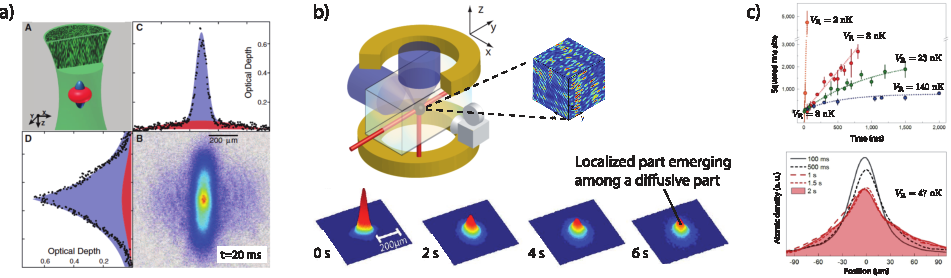
\includegraphics[width=\textwidth]{Fig/Localisation/localisation_3D_atomes_v1.pdf}
\caption{\textbf{Observation de la localisation d'Anderson à trois dimensions avec des atomes ultra-froids.} \textbf{a:} Localisation d'une partie du nuage de \isotope[40]{K} à temps très court. Une partie localisée émerge du centre d'un fond balistique. Figure tirée de \citep{kondov2011three}. \textbf{b:} Observation à temps très long d'une partie localisée du nuage de \isotope[87]{Rb} qui se démarque d'un fond très peu diffusif dans un désordre quasi-isotrope. Figure tirée de \citep{jendrzejewski2012three}. \textbf{c:} Localisation d'un nuage de \isotope[39]{K} complet dont les interactions sont annulées à l'aide d'une résonance de Feshbach. Figure tirée de \citep{semeghini2015measurement}.}
\label{fig:localisation_3D_atomes_froids}
\end{figure}





\paragraph*{Localisation dynamique}
Notons enfin l'existence d'un autre système permettant d'étudier la localisation d'Anderson à l'aide d'atomes froids, basé sur le phénomène de \emph{localisation dynamique}. Développé expérimentalement dans les années 1990 \citep{moore1995atom}, le système de \emph{rotateurs forcés} (ou \emph{kicked rotors} en anglais) repose sur un mapping entre un rotateur pulsé périodiquement et un modèle d'Anderson. Celui-ci se focalise sur l'apparition du phénomène de localisation dans l'espace des vitesses \citep{lemarietel-00424399}. 

En effet, à l'aide d'une onde stationnaire pulsée périodiquement, équivalente à une transmission périodique d'impulsion aléatoire, on peut décrire le mouvement des atomes soumis à ces \emph{kicks} comme une marche aléatoire dans l'espace des vitesses. Cependant, la richesse de ce système réside dans sa dynamique quantique, grâce à laquelle le phénomène de localisation apparaît de manière équivalente à celle dans l'espace réel et présente une localisation exponentielle de la distribution de vitesses des atomes illustrée figure \ref{fig:kicked_rotors}.

\begin{figure}
\centering
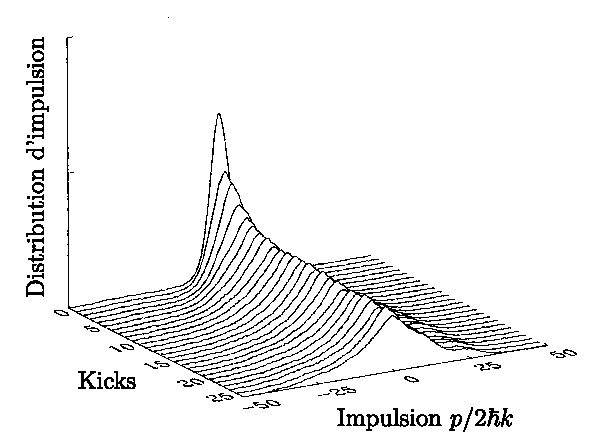
\includegraphics[width=0.6\textwidth]{Fig/Localisation/kicked_rotor.pdf}
\caption{\textbf{Localisation dynamique d'atomes froids.} Un nuage d'atomes de sodium est soumis à des kicks périodiques, induisant une marche aléatoire dans l'espace des impulsions. Après un certain nombre de kicks, la distribution d'impulsion se fige et présente une décroissance exponentielle. Figure tirée de \citep{moore1995atom}. }
\label{fig:kicked_rotors}
\end{figure}

L'extension du kicked rotor unidimensionnel à des dimensions supérieures $d=2$ et $d=3$ a pu se faire à l'aide d'une modulation temporelle des kicks \citep{casati1989anderson}. Le \emph{kicked rotor quasi-périodique} possède une transition de phase métal-isolant d'Anderson, confortée par l'existence d'un mapping \citep{lemarie2009observation} ainsi que par des études numériques \citep{lemarie2009universality}. L'expérience de Chabé et al. \citep{chabe2008experimental} réalisée à Lille rapporte ainsi une valeur de $\nu=1.63\pm0.05$ de l'exposant critique de la transition de phase associée, tout en vérifiant l'universalité de celle-ci \citep{lopez2012experimental}. Cette mesure constitue aujourd'hui encore la seule mesure expérimentale des exposants critiques de la transition d'Anderson compatible avec les estimations numériques \citep{slevin2014critical}.








\section{Vers l'étude du régime critique}
Nous avons vu dans la section précédente que la plateforme des atomes ultra-froids constitue un outil idéal pour étudier la problématique de la propagation cohérente d'ondes dans des milieux désordonnés. En revanche, malgré l'observation de la localisation d'Anderson dans des systèmes unidimensionnels ainsi que la transition d'Anderson dans des systèmes tridimensionnels, l'étude à énergie résolue de la transition d'Anderson reste un défi de taille auquel les trois expériences menées n'ont pas pu apporter de réponse.

Dans cette partie, nous allons donc décrire les manquements des différentes expériences afin de dresser un état de l'art de l'étude de la transition d'Anderson avec des atomes ultra-froids. Enfin, nous nous pencherons brièvement sur l'approche suivie par notre équipe pour tenter de dépasser ces limitations.

\subsection{Etat de l'art de l'étude de la transition d'Anderson avec des atomes ultra-froids}
\label{sc:etat_art_transition}
Comme nous allons le voir plus en détails, les trois expériences menées jusqu'à présent ont pour similarité d'estimer le seuil de mobilité à l'aide de la fraction localisée. La détermination précise du seuil de mobilité constitue une étape cruciale vers l'étude du régime critique de la transition d'Anderson. 

Contrairement aux exposants critiques de la transition d'Anderson, l'énergie critique de la transition, le seuil de mobilité, dépend des détails microscopiques du désordre. L'utilisation de désordres de type speckle par les expériences, de distribution asymétrique (voir chapitre \ref{ch:Speckle}), résultent en un comportement complexe du seuil de mobilité, qui diffère entre potentiels répulsifs ou attractifs. 


\paragraph*{Expérience d'Urbana Champaign}
La première expérience à donner une estimation du seuil de mobilité à l'aide d'atomes ultra-froids a été menée en 2011 à Urbana Champaign aux États-Unis \citep{kondov2011three}. Celle-ci se base sur l'expansion d'un nuage thermique de \isotope[40]{K} polarisé\footnote{Le \isotope[40]{K} est une espèce fermionique dont les collisions dans l'onde \textit{s} sont supprimées si les atomes se trouvent dans le même état de spin. On peut ainsi négliger les interactions entre atomes.} dans un speckle répulsif anisotrope. L'analyse des auteurs repose sur l'observation d'une double structure du profil de densité atomique pour des temps de propagation $t\geq \SI{20}{\milli\second}$, interprétée comme la coexistence d'états localisés et d'états diffusifs. En définissant la fraction localisée comme la rapport entre le nombre d'atomes localisés et le nombre d'atomes total $\floc=N_{\mathrm{loc}}/(N_{\mathrm{loc}}+N_{\mathrm{D}})$, il est possible d'estimer le seuil de mobilité en remarquant que seuls les atomes d'énergie inférieure à $\Ec$ restent localisés:
\begin{equation}
\floc=\int_{-\infty}^{\Ec}{\mathrm{d}E \: \DE} \text{ ,}
\label{eq:fraction_localisee}
\end{equation}
où $\DE$ est la distribution d'énergie des atomes dans le potentiel désordonné.

Afin de déterminer la distribution d'énergie $\DE$, les auteurs font l'hypothèse que l'allumage lent du désordre sur les atomes ne modifie par leur distribution d'énergie, alors déduite de la distribution des vitesses de Maxwell-Boltzmann. En introduisant la \emph{fonction spectrale}\footnote{Cette quantité est d'une importance capitale pour l'étude de la localisation d'Anderson avec des atomes froids. Elle sera étudiée plus en détails dans le chapitre \ref{ch:TauS_NJP}.} $A(\mathbf{k},E)$ représentant la probabilité qu'une particule d'impulsion $\mathbf{k}$ ait une énergie $E$ en présence de désordre
\begin{equation}
\DE= \int{\frac{\mathrm{d}^d \mathbf{k}}{{(2 \pi)}^d} \: A(\mathbf{k},E) \: \mathcal{D}_{\mathbf{k}}(\mathbf{k})} \text{ ,}
\label{eq:fonction_spectrale}
\end{equation}
l'hypothèse des auteurs selon laquelle le désordre n'affecte pas la distribution d'énergie des atomes revient à assimiler la fonction spectrale à une distribution infiniment fine:
\begin{equation}
A(\mathbf{k},E) = \delta\left(E- \frac{\hb^2 \mathbf{k}^2}{2m}\right) \text{ .}
\label{eq:hypothese_urbana_champaign}
\end{equation}

De nombreuses critiques ont été formulées quant à l'interprétation des données expérimentales \citep{muller2014comment}. Notamment, les très courts temps de propagation dans le désordre ne permettent pas de conclure quant à l'observation à proprement parler d'états localisés, indissociables d'états très lentement diffusifs. La fraction localisée extraite et le seuil de mobilité sont donc largement surestimés. De plus, l'observation de la localisation d'Anderson à trois dimensions requiert l'utilisation d'un désordre fort (comme spécifié par le critère de Ioffe-Regel $k\lb\sim 1$) pour lequel la distribution d'énergie $\DE$ est profondément modifiée. Les résultats de cette étude ne permettent donc pas de conclure quant à la mesure du seuil de mobilité \citep{pasek2017anderson}.



\paragraph*{Expérience de Palaiseau}
La seconde expérience, réalisée à Palaiseau en 2012, se focalise sur l'évolution temporelle de l'expansion d'un condensat de Bose-Einstein de \isotope[87]{Rb} dilué dans la superposition cohérente de deux speckles croisés afin d'obtenir un désordre quasi-isotrope \citep{jendrzejewski2012three}. Le suivi de la densité atomique $n(\mathbf{x},t)$ au cours de l'expansion jusqu'à \SI{6}{\second} témoigne d'une double structure pour les désordres les plus forts, identifiée à l'existence d'une partie localisée et d'un fond diffusif, comme illustré figure \ref{fig:experience_palaiseau}:
\begin{equation}
n(\mathbf{x},t)= \floc n_i(\mathbf{x}) + n_{\mathrm{D}}(\mathbf{x},t) \text{ .}
\end{equation}

L'estimation de la fraction localisée $\floc$ est réalisée en suivant la densité atomique au centre du nuage\footnote{Il s'agit en réalité de la densité atomique intégrée suivant la direction d'imagerie, voir section \ref{sc:imagerie}.}, ajustée par l'asymptote $\floc+\chi/t$, qui tient compte de la contribution de la partie diffusive aux temps longs, voir figure \ref{fig:experience_palaiseau}. L'utilisation d'une telle limite asymptotique permet ainsi de s'affranchir des temps de propagation finis.


Étant donné la très faible énergie des atomes, l'onde de matière initiale peut être considérée comme une onde plane $\etat{\mathbf{k}=0}$. Contrairement à l'expérience d'Urbana Champaign, le désordre est allumé brusquement, projetant ainsi l'état initial sur les différents états propres du désordre. À l'aide de l'équation \ref{eq:fonction_spectrale}, on trouve que la distribution d'énergie des atomes dans le désordre est donnée par 
\begin{equation}
\DE = A(\mathbf{k}=0,E) \text{ ,}
\end{equation}
calculée numériquement. Une fois la distribution d'énergie des atomes dans le désordre connue, il est possible d'estimer le seuil de mobilité à l'aide de l'équation \ref{eq:fraction_localisee} \citep{piraud2012localisation}.

Si l'observation de l'arrêt de l'expansion d'une partie du nuage est directe dans cette expérience, la détermination du seuil de mobilité est quant à elle très indirecte. En effet, celle-ci repose sur deux calculs intermédiaires: le calcul numérique de la fonction spectrale $A(\mathbf{k}=0,E)$ et le calcul de $\Ec$. 



\begin{figure}
\centering
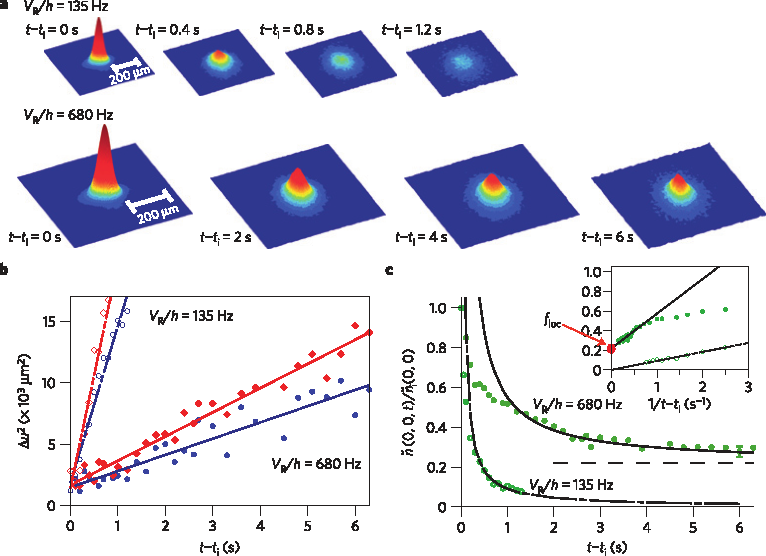
\includegraphics[width=\textwidth]{Fig/Localisation/experience_palaiseau.pdf}
\caption{\textbf{Expérience de Palaiseau.} \textbf{a:} Images expérimentales du nuage de \isotope[87]{Rb} après propagation dans le désordre. Pour un désordre de \SI{135}{\hertz}, le nuage a une dynamique de diffusion. Pour un désordre de \SI{680}{\hertz}, une partie localisée apparaît parmi un fond diffusif lent. \textbf{b:} Évolution temporelle de la taille du nuage selon deux axes. L'augmentation de l'amplitude du désordre ralentit la diffusion du nuage. \textbf{c:} Évolution de la densité atomique au centre du nuage. Le régime asymptotique (aux temps longs) permet de déterminer la fraction localisée. Figure tirée de \citep{jendrzejewski2012three}.}
\label{fig:experience_palaiseau}
\end{figure}


\paragraph*{Expérience de Florence}
La troisième expérience, réalisée en 2015 à Florence, est la dernière expérience en date cherchant à déterminer le seuil de mobilité avec des atomes ultra-froids \citep{semeghini2015measurement}. Si celle-ci partage de nombreuses similarités avec les expériences précédentes, telles que l'utilisation d'un désordre de type speckle répulsif et l'estimation du seuil de mobilité à l'aide de la mesure de la fraction localisée, elle se distingue par l'approche utilisée pour peupler les différents états. 

En effet, l'originalité de cette expérience est de moduler l'amplitude du potentiel pendant \SI{500}{\milli\second} afin de transférer une partie contrôlée des atomes initialement dans un état d'énergie $E$ à un état d'énergie $E+\hb \omega$ avec $\omega$ la fréquence de modulation. La fraction localisée est ensuite obtenue en détectant les atomes localisés après \SI{500}{\milli\second} supplémentaires de propagation dans le désordre, voir figure \ref{fig:experience_florence}. De manière identique aux expériences précédentes, le seuil de mobilité est déterminé à l'aide de l'équation \ref{eq:fraction_localisee}.

\begin{figure}
\centering
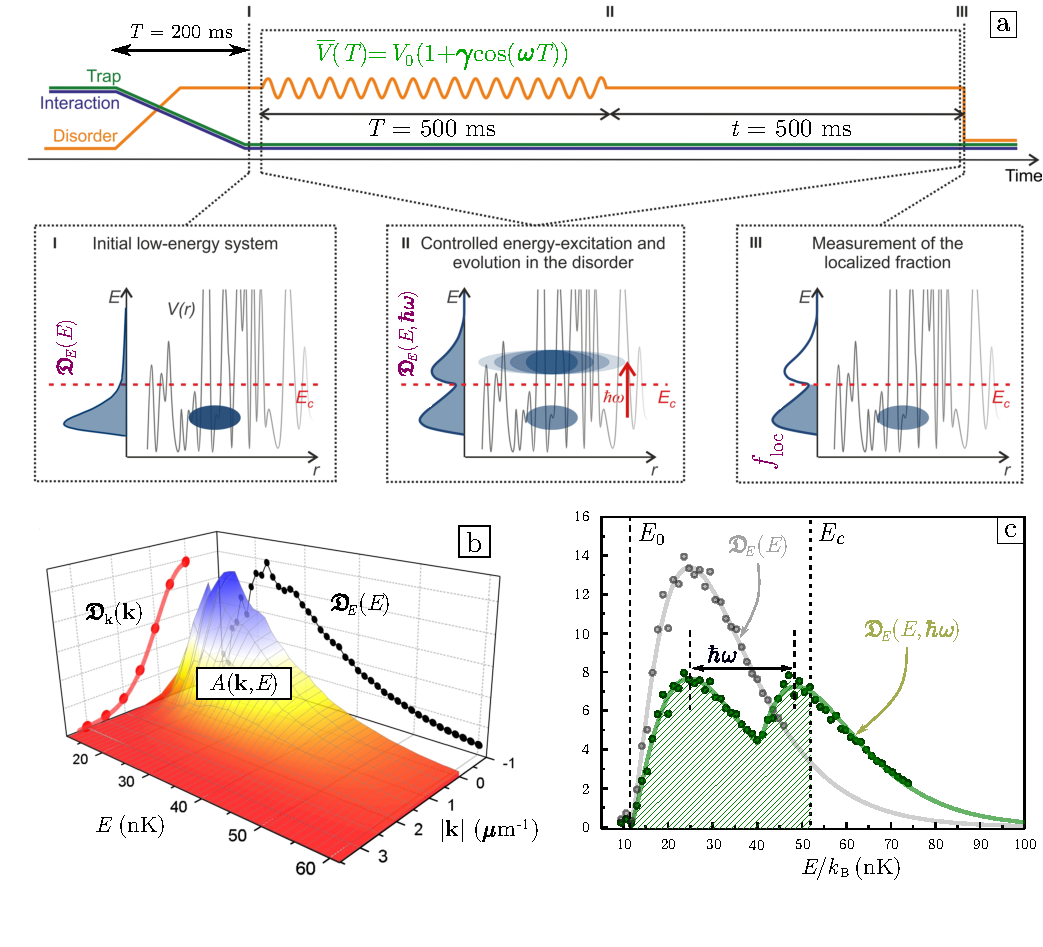
\includegraphics[width=\textwidth]{Fig/Localisation/experience_florence.pdf}
\caption{\textbf{Expérience de Florence.} \textbf{a:} Procédure de mesure du seuil de mobilité. Un état de basse énergie est chargé dans le désordre. Une modulation de l'amplitude du désordre permet de transférer une énergie $\hb \omega$ à certains atomes. La propagation dans le désordre permet d'éliminer la partie diffusive, révélant ainsi la fraction localisée. \textbf{b:} Fonction spectrale $A(\mathbf{k},E)$ calculée numériquement. Celle-ci permet de calculer la distribution d'énergie des atomes dans le désordre à partir de la distribution d'impulsion des atomes mesurée après le chargement du désordre. \textbf{c:} Exemple de distribution d'énergie des atomes après chargement, modulation et propagation dans le désordre. La courbe grise correspond à la distribution d'énergie après chargement du désordre, la courbe verte correspond à la distribution d'énergie après modulation de l'amplitude du désordre et la surface verte correspond à la fraction des atomes qui sont localisés. Figure tirée de \citep{denechaud2018vers}.}
\label{fig:experience_florence}
\end{figure}

Une seconde distinction avec l'expérience de Palaiseau réside dans la procédure de chargement du désordre. En effet, le désordre est ici allumé progressivement et la distribution d'impulsion du nuage $\mathcal{D}_{\mathbf{k}}(\mathbf{k})$ n'est plus associée à l'onde plane $\etat{\mathbf{k}=0}$. Ainsi, la distribution d'énergie des atomes dans le désordre est donnée par l'équation \ref{eq:fonction_spectrale}, où la distribution d'impulsion est mesurée expérimentalement par la méthode de temps de vol et la fonction spectrale est calculée numériquement. La détermination de la distribution d'énergie nécessite donc de calculer la fonction spectrale pour toutes les impulsions du nuage.

L'expérience de Florence se caractérise donc par une nouvelle approche à la mesure du seuil de mobilité. En particulier, l'attention portée à la sélection de l'énergie des atomes marque le début de l'étude de la transition d'Anderson à \emph{énergie résolue}. Néanmoins, cette expérience comporte des limitations. Notamment, la détermination du seuil de mobilité reste indirecte: il est nécessaire de calculer numériquement la fonction spectrale $A(\mathbf{k},E)$ ainsi que la population transférée. 



\paragraph*{Comparaison aux résultats numériques}
Les trois expériences présentées précédemment \citep{kondov2011three}\citep{jendrzejewski2012three}\citep{semeghini2015measurement} ont toutes cherché à montrer l'existence d'un seuil mobilité séparant les états localisés des états diffusifs. Pour cela, celles-ci se sont basées sur la mesure de fractions localisées et sur des estimations de la distribution d'énergie des atomes dans le désordre.

Un second point commun entre ces expériences réside dans la nature du désordre utilisé: toutes ont utilisé un speckle répulsif, généré à l'aide d'un unique faisceau pour l'expérience d'Urbana Champaign tandis que les expériences de Palaiseau et de Florence ont profité de l'interférence de deux speckles croisés pour générer un désordre quasi-isotrope. 

Dans le cadre de l'étude de l'effet de l'anisotropie du potentiel sur la position du seuil de mobilité pour un potentiel de type speckle, Pasek et al. \citep{pasek2017anderson} ont montré qu'il existe une échelle d'énergie universelle, appelée \emph{énergie de corrélation}, qui rend la position du seuil de mobilité indépendante des longueurs de corrélation du désordre. Cette énergie est définie par
\begin{equation}
\ER=\frac{\hb^2}{m\overline{\sigma}^2} \quad \text{avec} \quad \overline{\sigma}={(\sigma_x \sigma_y \sigma_z)}^{1/3} \text{ ,}
\end{equation}
où les $\sigma_i$ correspondent aux longueurs de corrélation selon chaque direction.

À l'aide de cette définition, Pasek et al. ont pu comparer les résultats des différentes expériences à une unique courbe universelle $\Ec/\VR=\mathcal{F}(\VR/\ER)$ obtenue à l'aide de simulations numériques. La compilation de ces résultats est illustrée figure \ref{fig:seuil_mobilite_delande}.


\begin{figure}
\centering
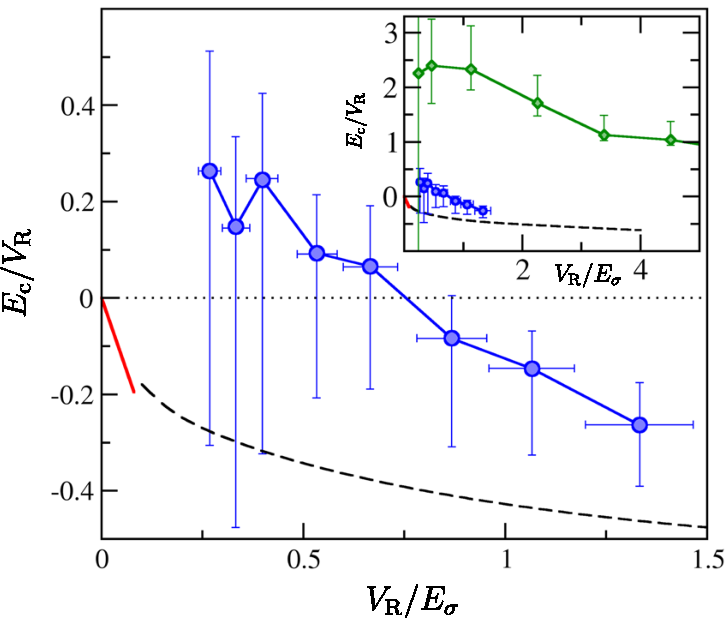
\includegraphics[width=0.6\textwidth]{Fig/Localisation/delande_expvsth.pdf}
\caption{\textbf{Comparaison des résultats expérimentaux à des simulations numériques.} Evolution du seuil de mobilité $\Ec$ en fonction de l'amplitude du désordre $\VR$. La ligne pointillée noire correspond à la prédiction universelle $\Ec/\VR=\mathcal{F}(\VR/\ER)$. Les résultats de l'expérience de Palaiseau sont représentés par la ligne rouge, tandis que les résultats de l'expérience de Florence sont reportés par des points bleus. Les résultats de l'expérience d'Urbana Champaign sont représentés par des points verts dans l'encart. Figure tirée de \citep{pasek2017anderson}.}
\label{fig:seuil_mobilite_delande}
\end{figure}

Les résultats de l'expérience d'Urbana Champaign, en points verts dans l'encart, montrent un désaccord significatif avec les résultats numériques. En particulier, les résultats expérimentaux surestiment fortement le seuil de mobilité en raison du très court temps de propagation dans le désordre et de l'hypothèse \ref{eq:hypothese_urbana_champaign}. L'expérience de Palaiseau, dont les résultats sont représentés en rouge, semblent en accord quantitatif avec les prédictions numériques. Les résultats de l'expérience de Florence sont représentés en bleu et semblent en accord qualitatif avec les résultats numériques. Néanmoins, les données expérimentales semblent légèrement surestimer le seuil de mobilité, probablement en raison d'un temps de propagation trop court dans le désordre ou du calcul de la distribution d'énergie. L'ensemble de ces résultats montre donc qu'il est fondamental d'avoir des temps de propagation dans le désordre de plusieurs secondes afin de ne pas surestimer le seuil de mobilité.




\subsection{Nécessité d'une spectroscopie pour sonder le régime critique}
Les trois expériences citées précédemment reposent sur une détermination indirecte du seuil de mobilité, et nécessitent une estimation numérique de la distribution d'énergie $\DE$, capitale pour calculer le seuil de mobilité. Comme nous l'avons vu, l'obtention de la distribution d'énergie passe par l'intermédiaire de la fonction spectrale $A(\mathbf{k},E)$, qu'aucune de ces expériences n'a mesurée. 

De plus, dans le cas d'une estimation fiable de la fonction spectrale, la coexistence d'une phase localisée et d'une phase diffusive témoigne d'une large distribution d'énergie, rendant l'étude du régime critique et plus particulièrement des exposants critiques de la transition impossible.

Il apparaît donc que, dans l'optique de sonder le régime critique, il est important de maîtriser le paramètre de contrôle de la transition d'Anderson, c'est à dire l'énergie $E$ de l'onde. Pour cela, une nouvelle approche expérimentale résolue en énergie s'avère nécessaire, approche pour laquelle il est possible de peupler sélectivement les états $\etat{E}$ d'énergie bien définie du désordre. Il s'agit donc de réaliser une spectroscopie du désordre.





Le protocole expérimental de spectroscopie de la transition d'Anderson est proche de celui de l'expérience de Florence: un état initial $\etat{i}$ libre de faible énergie est transféré sélectivement dans un état propre $\etat{E_\alpha}$ du désordre dans un premier temps, puis une expansion de plusieurs secondes dans le désordre permet de déterminer si cet état est localisé, ou non. 




\begin{figure}
\centering
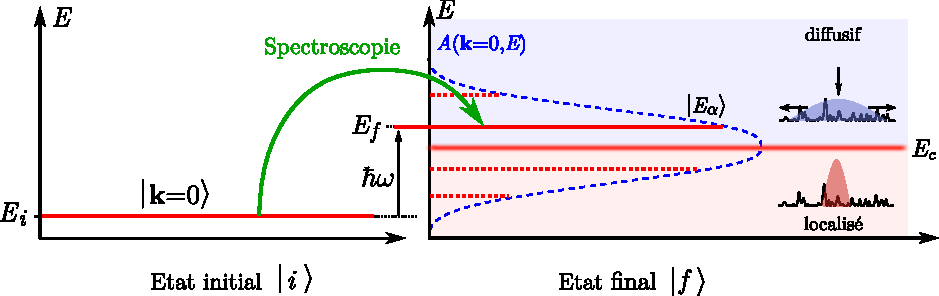
\includegraphics[width=\textwidth]{Fig/Localisation/spectroscopie_anderson.pdf}
\caption{\textbf{Approche spectroscopique de l'étude la transition d'Anderson.} Dans l'optique de sonder la transition d'Anderson, il est nécessaire de peupler sélectivement les différentes énergies du désordre. Pour cela, l'onde est préparée dans un état insensible au désordre, puis est transférée à une énergie bien définie dans le désordre à l'aide d'une spectroscopie. Enfin, l'expansion du nuage permet de caractériser l'énergie adressée en terme de localisation ou de diffusion.}
\label{fig:spectroscopie_anderson}
\end{figure}


Depuis ces premiers résultats expérimentaux novateurs, la mise en place d'une telle spectroscopie sur notre expérience a permit de mesurer les fonctions spectrales $A(\mathbf{k}=0,E)$ (le protocole de mesure sera explicité dans le chapitre \ref{ch:TauS_NJP}), démontrant notre capacité à adresser des énergies spécifiques dans le désordre \citep{volchkov2018measurement}. Cependant, différentes limitations expérimentales ont empêché de procéder aux mesures d'expansion nécessaires à la caractérisation des différents états d'énergie en terme de localisation. Les deux principales sources de limitation identifiées seront discutées dans les chapitres \ref{ch:new_exp} et \ref{ch:Speckle}.


\begin{comment}

%%% mettre les performances ??? ceci peut être intéressant ? chercher données ? Freedman peut être ?
\begin{figure}[h!]
	\centering
	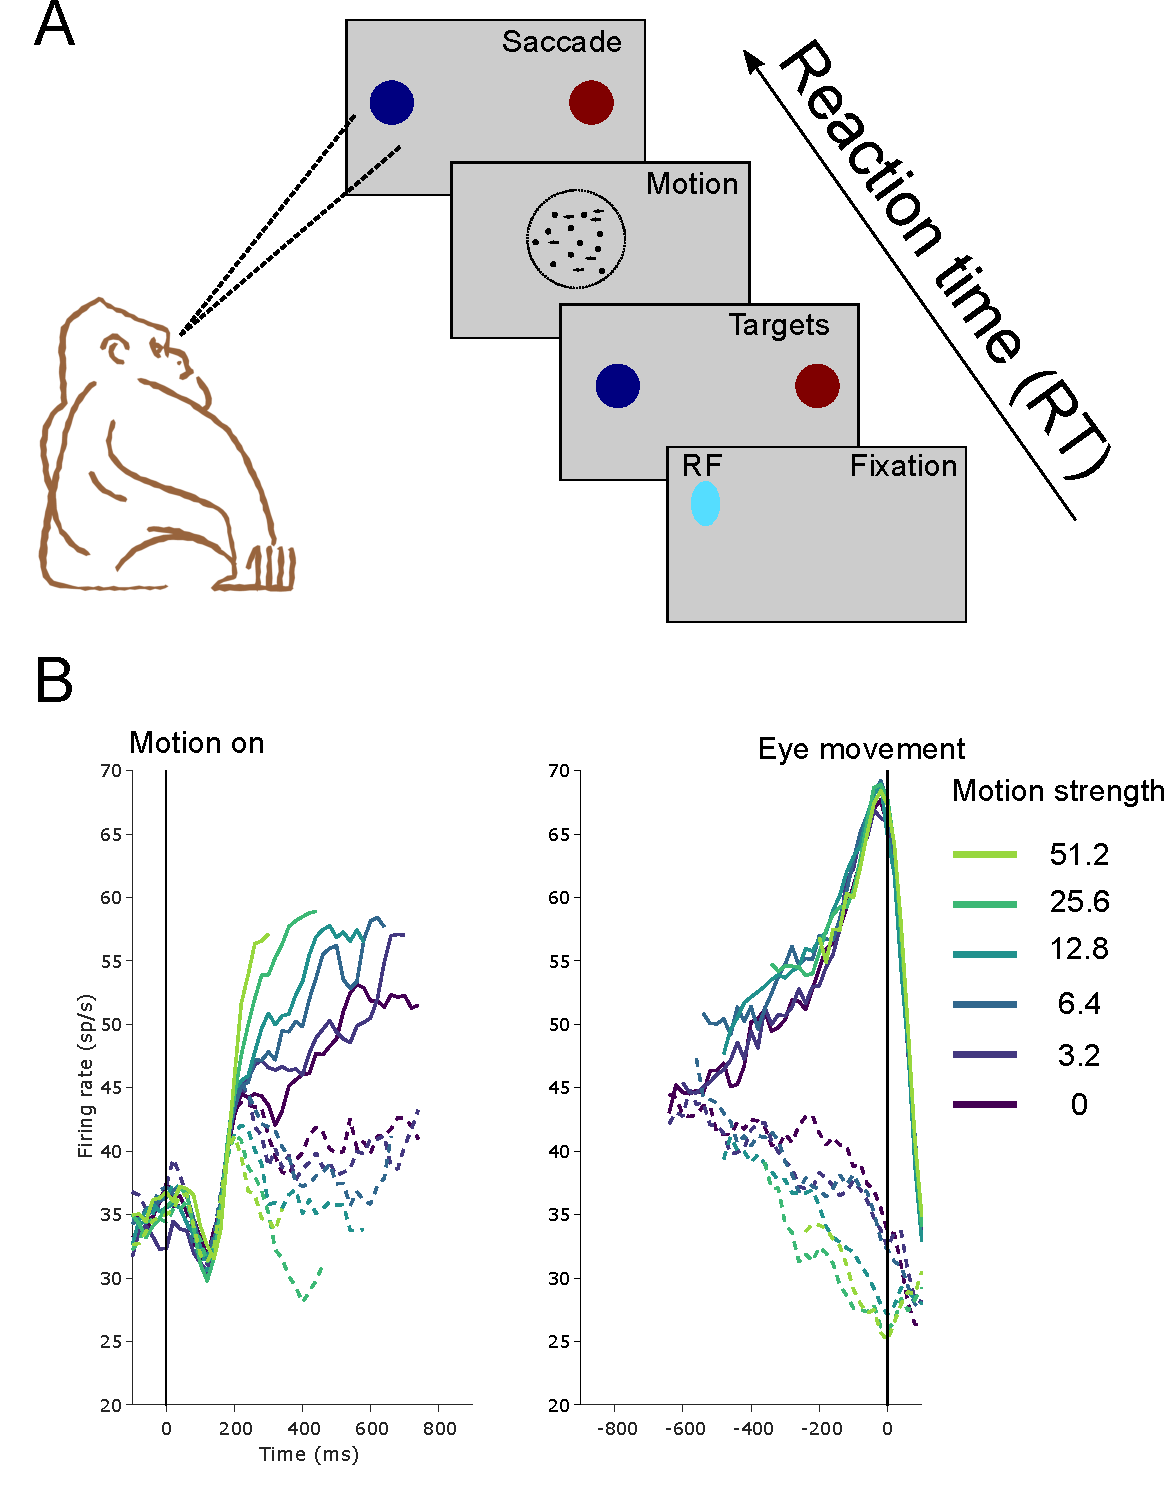
\includegraphics[width=0.8\linewidth]{Fig/Chapter1/RDM.pdf}
	\caption{{\bf Reaction time version of the random dot motion discrimination task.}   (A) The monkey views a set of dots moving across the screen and decides the net direction of movement. The decision is indicated by a saccadic eye movement to one the two peripheral target. The light blue field corresponds to the receptive field of one of the recorced LIP neurons. The monkey is the figure was obtained using the AutoDraw software. (B) Response of LIP neurons during decision. The data are from~\cite{roitman2002response} and are publicly available. The average firing rate of $54$ LIP neurons is shown for $6$ degrees of difficulty. The firing rate are grouped by motion difficulty and direction of choice (dashed line corresponding to choice out of the receptive field of the neuron). The left panel represents the average firing rate during decision formation starting from motion onset. The right panel shows the average firing rate centered at the time of the eye movement.
	}
	\label{fig:RDM}
\end{figure}
%% REF AutoDraw ??,

\end{comment}